\section{Returning to the original density}
\label{sec:density}

We now remove the factor $L$ in Proposition~\ref{prop:half-density}.
The useful coupling makes each row a product sample, while arranging
its dependence with the other rows so that their union has a larger
prescribed density.

\begin{proof}[Proof of Theorem~\ref{thm:main}]
Set $L=2^{70}$ and $k=32L=2^{75}$, and suppose that
$\mu_p(\mathcal D)\ge1-1/k$. In particular, $\mathcal D$ is nonempty.
We construct $L$ random sets $R_1,\ldots,R_L$, each with law $\mu_p$.
For any such construction the union bound gives
\begin{equation}
\label{eq:all-good-rows}
\mathbb P(R_j\in\mathcal D\text{ for all }1\le j\le L)
\ge1-\sum_{j=1}^L\mathbb P(R_j\notin\mathcal D)
\ge1-\frac Lk=\frac{31}{32}.
\end{equation}
Independence between rows is not required.

\medskip
\noindent\emph{Case 1: $Lp<1$.}
For each coordinate $i$, independently across coordinates, choose a label
$J_i\in\{0,1,\ldots,L\}$ with
\[
\mathbb P(J_i=0)=1-Lp,
\qquad
\mathbb P(J_i=j)=p\quad(1\le j\le L).
\]
Put $R_j=\{i:J_i=j\}$. For a fixed row $j$, its membership indicators
are independent Bernoulli variables of parameter $p$, so $R_j$ has law
$\mu_p$. The union $R=R_1\cup\cdots\cup R_L$ has law $\mu_q$,
where $q=Lp\in(0,1)$: a coordinate belongs to $R$ precisely when
its label is nonzero.
Figure~\ref{fig:coupling} illustrates the construction with three rows.

\begin{figure}[!ht]
\centering
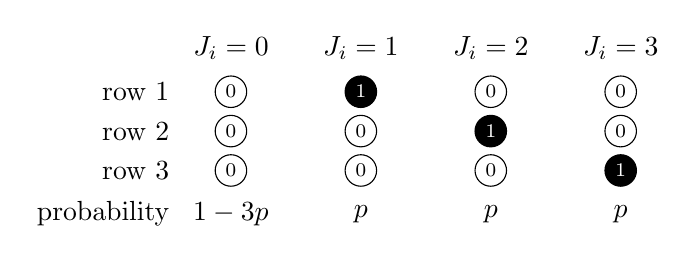
\begin{tikzpicture}[x=1.65cm,y=0.5cm,
  bit/.style={circle,draw,minimum size=4mm,inner sep=0pt},
  present/.style={bit,fill=black,text=white}]
  \foreach \x/\y in {0/1,0/2,0/3,1/1,1/2,2/1,2/3,3/2,3/3}
    \node[bit] at (\x,\y) {\scriptsize 0};
  \foreach \x/\y in {1/3,2/2,3/1}
    \node[present] at (\x,\y) {\scriptsize 1};
  \node at (0,4.1) {$J_i=0$};
  \node at (1,4.1) {$J_i=1$};
  \node at (2,4.1) {$J_i=2$};
  \node at (3,4.1) {$J_i=3$};
  \node at (0,-0.1) {$1-3p$};
  \foreach \x in {1,2,3} {\node at (\x,-0.1) {$p$};}
  \node[anchor=east] at (-0.4,3) {row 1};
  \node[anchor=east] at (-0.4,2) {row 2};
  \node[anchor=east] at (-0.4,1) {row 3};
  \node[anchor=east] at (-0.4,-0.1) {probability};
\end{tikzpicture}
\caption{One coordinate of the sparse coupling, illustrated with three
rows and $3p<1$. Each row contains this coordinate with probability $p$;
the union contains it with probability $3p$. Making these choices
independently across coordinates gives the required product laws.}
\label{fig:coupling}
\end{figure}


Define
\[
\mathcal F
=\{D_1\cup\cdots\cup D_L:D_1,\ldots,D_L\in\mathcal D\}.
\]
On the event in~\eqref{eq:all-good-rows}, the union $R$ belongs to
$\mathcal F$. Hence
\[
\mu_q(\mathcal F)=\mathbb P(R\in\mathcal F)
\ge\frac{31}{32}\ge\frac12.
\]
Grouping a tuple of $32L$ members of $\mathcal D$ into 32 groups of
size $L$, or conversely expanding 32 members of $\mathcal F$, shows that
the possible unions agree exactly. Thus
\[
E_{32}(\mathcal F)=E_{32L}(\mathcal D)=E_k(\mathcal D).
\]
Proposition~\ref{prop:half-density} makes this family $(q/L)$-small.
Since $q/L=p$, this is the required conclusion.

\medskip
\noindent\emph{Case 2: $Lp\ge1$.}
Set
\[
t=\frac{p-1/L}{1-1/L}\in[0,1).
\]
At each coordinate $i$, choose a mandatory row uniformly among the $L$
rows. Include $i$ in that row, and, conditional on this choice, include
it independently in each other row with probability $t$.
Make these choices independently across coordinates. For each fixed
row $j$,
\[
\mathbb P(i\in R_j)
=\frac1L+\left(1-\frac1L\right)t=p,
\]
and the coordinates of $R_j$ are independent. Thus each $R_j$ again has
law $\mu_p$, while the union of all rows is $[N]$ in every outcome.

By~\eqref{eq:all-good-rows}, some outcome has all $L$ rows in
$\mathcal D$. These rows cover $[N]$. Repeating the resulting tuple
32 times gives exactly $k$ members of $\mathcal D$ with full union.
Consequently $E_k(\mathcal D)=\varnothing$, which is covered at cost
zero by the empty family. This construction also covers the boundary
$Lp=1$, when $t=0$.
\end{proof}
